%\part{}
\lecture{Introduction to Bivariate Data}{introduction-to-bivariate-data}


\title{Introduction to Bivariate Data}
\subtitle{Qualitative and Quantitative Data}

\author{Kelly Black}
\institute{Clarkson University}
\date{23 January 2012}

\begin{frame}
  \titlepage
\end{frame}

\begin{frame}
  \frametitle{Outline}
  \tableofcontents[pausesection,hideallsubsections]
\end{frame}


\section{Clicker Quiz}


\begin{frame}
  \frametitle{Clicker Quiz}

  We have a data set and find a sample mean of 2.5 and a sample
  standard deviation of 6.1. What is the $z$-statistic for $x=2.7$.

  \begin{tabular}{l@{\hspace{3em}}l@{\hspace{3em}}l@{\hspace{3em}}l}
    A: -1.220 & B: -0.033 & C: 0.033 & D: 1.220
  \end{tabular}


\end{frame}




\section{Bivariate Data}

\begin{frame}
  \frametitle{Bivariate Data}

  \begin{eqnarray*}
    \begin{array}{l|l}
      x      & y \\ \hline 
      x_1    & y_1 \\
      x_2    & y_2 \\
      \vdots & \vdots \\
      x_n    & y_n
    \end{array}
  \end{eqnarray*}
\end{frame}

\section{Qualitative Data}

\begin{frame}
  \frametitle{Cross Tabular Tables}

  \begin{tabular}{ll}
    $Q_{1}$ & $Q_{2}$ \\ \hline
    A & Y \\
    B & Y \\
    B & N \\
    B & N \\
    A & N \\
    B & N
  \end{tabular}

  \uncover<2->
  {
    \begin{tabular}{l|l|l|l}
      $Q_1 \backslash Q_2$ & Y & N & Row Total \\
      A & 1 & 1 & 2 \\ \hline
      B & 1 & 3 & 4 \\ \hline
      Col. Total & 2 & 4 & 6
    \end{tabular}
  }

\end{frame}


\begin{frame}
  \frametitle{Clicker Quiz}


  Determine the table for this data with the row percentages:

  \begin{columns}
    \column{.25\textwidth}

  \begin{tabular}{l|l}
    $Q_{1}$ & $Q_{2}$ \\ \hline
    a & d \\
    a & e \\
    b & e \\
    a & d \\
    b & e \\
    a & d
  \end{tabular}


    \column{.75\textwidth}

    1:
    \begin{tabular}{l|l|l|l}
      $Q_1 \backslash Q_2$ & d & e & Row \\
      a & 3/4 & 1/4 & 1.0 \\ \hline
      b & 0.0 & 1.0 & 1.0 \\ \hline
      Col.  & 3/6 & 3/6 & 1.0
    \end{tabular}

    \rule{5cm}{0.05cm}

    2:
    \begin{tabular}{l|l|l|l}
      $Q_1 \backslash Q_2$ & d & e & Row  \\
      a & 1.0 & 1/3 & 4/6 \\ \hline
      b & 0.0 & 2/3 & 2/6 \\ \hline
      Col.  & 1.0 & 1.0 & 1.0
    \end{tabular}

    \rule{5cm}{0.05cm}

    3:
    \begin{tabular}{l|l|l|l}
      $Q_1 \backslash Q_2$ & d & e & Row  \\
      a & 1.0 & 0.0 & 1.0 \\ \hline
      b & 1/3 & 2/3 & 1.0 \\ \hline
      Col.  & 3/5 & 2/5 & 1.0
    \end{tabular}


  \end{columns}

\end{frame}

\section{Quantitative Data}

\begin{frame}
  \frametitle{Quantitative Data}

  \begin{eqnarray*}
    \begin{array}{l|l}
      X & Y \\ \hline
      x_1 & y_1 \\
      x_2 & y_2 \\
      x_3 & y_3 \\
      x_4 & y_4 \\
      \vdots & \vdots \\
      x_n & y_n
  \end{array}
\end{eqnarray*}

\end{frame}

\begin{frame}
  \frametitle{Example}

  \begin{columns}
    \column{.25\textwidth}

  \begin{eqnarray*}
    \begin{array}{r|r}
      X & Y \\ \hline
      3 & 6 \\
      2 & 2 \\
      -1 & -3 \\
      4 & 4 \\
      2 & 3
    \end{array}
  \end{eqnarray*}


    \column{.75\textwidth}

  \only<2->
  {
    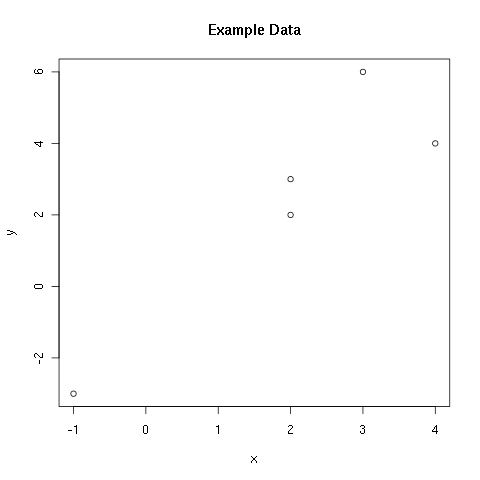
\includegraphics[width=7cm]{img/simpleBivariateExample}
  }


  \end{columns}


\end{frame}


% LocalWords:  Clarkson pausesection hideallsubsections Bivariate
